\chapter[SCP-089 托非特]{
    SCP-089 Tophet\\
    SCP-089 托非特
}

\label{chap:SCP-089}

\begin{figure}[H]
    \centering
    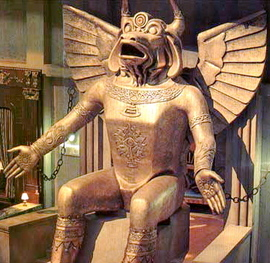
\includegraphics[width=0.5\linewidth]{images/SCP-089.jpg}
    \caption*{\bb{SCP-089},被运到了SCP-089-B的居所地以执行M8程序。}
\end{figure}

\bb{项目编号:}SCP-089

\bb{项目等级:}Euclid(见下)

\bb{特殊收容措施:}SCP-089储存在一个位于Site-36的特殊的集装箱内,对其采取了监控措施以监控叙事事件的发生。已建立起了一支由一些受过高级语言学、心理学和战术谈判培训的员工组成的机动特遣队Mu-89来对应对上述的叙事事件。当发生叙事事件时,机动特遣队Mu-89需翻译并理解该叙述以确定引发事件的主要对象(文中编为SCP-089-A和SCP-089-B),随后实施M8程序,此程序由以下几步组成:

\begin{enumerate}
\item 将SCP-089运至SCP-089-A的所在地,随后将M8程序向SCP-089-B进行解释;然后
\item 在SCP-089-B准备自愿执行M8程序的情况下,向SCP-089-B可能会提出的与SCP-089-B将进行的下列行动相关的要求给予一切协助:将SCP-089-A和例如油浸木材或木炭等易燃物一起放入洞中,然后点燃。
\end{enumerate}

M8程序的成功执行需要SCP-089-B在头脑清醒且未被强迫情况下的自愿合作。同样地,SCP-089-A也必须在程序实施过程中清醒且警觉。鉴于程序的过程对SCP-089-A来说极为痛苦并将最终毁灭SCP-089-A,建议在点火之后使SCP-089-A保持镇静(但不能睡着)以防止出现对程序的妨碍。

如果由于SCP-089-B不认可上述的说明来自愿执行M8程序,机动特遣队Mu-89需向其解释未完成程序将导致的情况,并且需尽一切努力来说服SCP-089-B合作。若机动特遣队Mu-89即使进了最大努力也未能说服SCP-089-B,则需将SCP-089重编为Keter级别,随后执行M9程序(参考文件089-M9)。绝对禁止使用恐吓、威胁、致幻剂和致醉物来影响SCP-089-B的自由意愿的,或任何尝试不借助SCP-089-B的参与或自愿合作的,或使用除上述正确方法外的任何方法的行为,因为这些举动将使前期对完成程序的努力前功尽弃,且已证明会增强随之发生的S型事件的严重性。

同时建议(虽不是M8程序的必要部分之一)在M8程序第二步的执行过程中,最好用喇叭声和击打乐器声作为伴奏,这样会掩盖SCP-089-A在执行程序过程中发出的声音。

当一次M8程序圆满完成后,相关的S型事件一般会在7小时内减弱。

\bb{描述:}SCP-089是一个上过釉的陶制雕像,大约有3米高,所塑的是一个有翅膀并张着嘴的牛头人。雕像的前躯干有铰链连接,可从顶部打开,里面是一个也可从外面锁上的洞,其容积大约是0.6立方米。雕像的背面有一段迦南语(或古迦太基语)的说明。\footnote{原注:██████博士翻译了文中的一段:“噩梦般的摩洛克!缺乏爱的摩洛克!精神摩洛克!摩洛克人类无情的审判官!”}雕像的历史可追溯到大约公元前2世纪。

罕见情况下(有时出现的间隔甚至有一个多世纪),该雕像会讲话。现仍未弄清这些声音产生的机制,讲话时雕像的嘴也不动。雕像的口音属于迦南语(或许与上述说明是同一语言),由下列内容组成:

\begin{itemize}
\item SCP-089-A的名字或描述;
\item 对完成M8程序的要求,同时还有对如何做的指示;和
\item 通过比喻的方法对相关的S型事件进行的描述
\end{itemize}

每个叙事事件过后的三至十一天内,之前描述过的S型事件都会开始发生,除非M8程序已顺利完成。S型事件都是瘟疫、自然灾害、种族灭绝狂热或者其他大屠杀一类的事件,或者是一些一直持续到M8程序顺利完成才停止的造成了大量财产、人员损失的事件。在所有记录下来的叙事事件中,伴随着S型事件虽然都产生了重大影响,但,这类事件发生的区域无法直接影响到SCP-089-B。故在一些案例中,由于SCP-089-B对SCP-089或M8程序的不了解,或者SCP-089-B不愿执行M8程序来停止S型事件,导致了S型事件持续了很长一段时间无法解决。

每个叙事事件中提到的SCP-089-A都是一个健康的、无缺陷的人类婴幼儿或孩童,年龄从八个月到六岁间不等,SCP-089-B则是孩子的亲生母亲。在所有已记载的案例中,叙事事件发生的时候,SCP-089-A和-B都活着并很健康,彼此之间都十分信任和喜爱。

当SCP-089-B把SCP-089-A放在洞里然后点燃易燃材料后,在随后的二至五个小时内,SCP-089-A将会燃烧并将最终毁灭。

\bb{附录\#1:}\\
Garcia博士对文档的备忘:虽然现仍未知SCP-089在S型事件中起到什么作用,但之前的经验印证了迅速且规范地应用M8程序将很有效地减轻S型事件所造成的损失。Patel博士推测SCP-089并不会引发S型事件,而仅仅是预感到了事件将要发生,随后提供一种减轻事件效应的方法。

\bb{附录\#2:}\\
下面列出了一部分记录在案的通过M8程序最终消除了的S型事件(包括了有记载的在基金会将SCP-089纳入收容之前发生并完成了M8程序的):

\begin{scpbox}

\bb{叙述日期:}1788年3月16日\\
\bb{叙事事件中对S型事件的描述}“火将噬其房屋,继而,其市,其庙,其屋尽为火所噬,其将瞬亡。”\\
\bb{S型事件:}███ ███████的城市大火。\\
\bb{结果:}M8程序于叙事事件后第29天完成。该城66\%的建筑被摧毁。

\end{scpbox}

\begin{scpbox}

\bb{叙述日期:}1850年12月2日\\
\bb{叙事事件中对S型事件的描述:}“有传道者,冒先知之名,行乡间以聚众,惑民攻上。尸横盈野,乡民十去八九;丁户尽丧,田不出斗升。”\\
\bb{S型事件:}█████的大规模以救世主自居的农民起义。\\
\bb{结果:}M8程序于叙事事件后第1363天完成。在起义和镇压过程中发生的大屠杀,和随后带来的农业崩溃共导致了至少██百万人的死亡。

\end{scpbox}

\begin{scpbox}

\bb{叙述日期:}1951年11月23日\\
\bb{叙事事件中对S型事件的描述:}“地山迸海沸,地火出于山,东海漫于野,声振寰宇,暗日而咽星,生屠而死猖。”\\
\bb{S型事件:}████的地震和火山喷发。\\
\bb{结果:}M8程序于叙事事件后31小时内被执行。虽地质模型推测此区域发生的地震将引发海啸,但最终未产生海啸。没有导致严重的损失。

\end{scpbox}

\begin{scpbox}

\bb{叙述日期:}1970年11月7日\\
\bb{叙事事件中对S型事件的描述:}“天河倾覆,湖川泛滥,人不能存,牲畜四载皆为所毁。”\\
\bb{S型事件:}██████████的飓风。\\
\bb{结果:}M8程序于叙事事件后第49天被执行。洪水、疾病和饥饿造成了███千人的死亡。

\end{scpbox}

\begin{scpbox}

\bb{叙述日期:}20██年4月4日\\
\bb{叙事事件中对S型事件的描述:}{[}数据删除]\\
\bb{S型事件:}{[}数据删除]\\
\bb{结果:}正在发生。M8程序尚未被执行。

\end{scpbox}
